\documentclass{article}
\usepackage[utf8]{inputenc}
\usepackage[english]{babel}
\usepackage[]{amsthm} %lets us use \begin{proof}
\usepackage[]{amssymb} %gives us the character \varnothing
\usepackage{amsmath,enumerate,float,graphicx,mathtools,minted,relsize,xlop}
\usepackage[margin=1in]{geometry} 
\usepackage{amsfonts, fancyhdr, color, comment, environ}
\usepackage{xcolor}
\usepackage{mdframed}
\usepackage[shortlabels]{enumitem}
\usepackage{indentfirst}
\usepackage{hyperref}
\hypersetup{
    colorlinks=true,
    linkcolor=blue,
    filecolor=magenta,      
    urlcolor=blue,
}

\newenvironment{problem}[2][]
    { \begin{mdframed}[backgroundcolor=gray!20] \textbf{#1#2} \\}
    {  \end{mdframed}}

% Define solution environment
\newenvironment{solution}
    {\textit{Solution:}\\}
    {$\blacksquare$}
  
\renewcommand{\qed}{\quad\qedsymbol}

% prevent line break in inline mode
\binoppenalty=\maxdimen
\relpenalty=\maxdimen

\newcommand{\bb}{\mathbf}
\newcommand{\unitvector}[2]{%
  \mathop{}\!\mathbf{#1}%
}
\newcommand{\ih}{\unitvector{i}}
\newcommand{\jh}{\unitvector{j}}
\newcommand{\kh}{\unitvector{k}}

\newcommand{\pd[1]}{\dfrac{\partial}{\partial #1}}
\newcommand{\pds[1]}{\dfrac{\partial^2}{\partial #1^2}}
\newcommand{\pdm[2]}{\dfrac{\partial^2}{\partial{#2}\partial{#1}}}
\newcommand{\pdf[2]}{\dfrac{\partial {#1}}{\partial {#2}}}

\newcommand{\pr}[1]{\left(#1\right)}
\newcommand{\vr}[1]{\left\langle#1\right\rangle}

\title{Midterm}
\author{Taylor Grover}
\date\today
%This information doesn't actually show up on your document unless you use the maketitle command below

\begin{document}
\maketitle %This command prints the title based on information entered above

%Section and subsection automatically number unless you put the asterisk next to them.
\begin{problem}{1. (20 points) decision tree}
For the data set at 
https://archive.ics.uci.edu/ml/datasets/Tic-Tac-Toe+Endgame
do the following:
\begin{enumerate}[{(}a{)}]
  \item Build a decision tree using ID3 for the whole data set.
  Give the tree in some human-readable format.
\end{enumerate}
\end{problem}
\begin{solution}
Using numpy in Python, the decision tree is constructed with the ID3 
algorithm, and the attributes are selected based on their total
information gain. The get\_information\_gain function throws 
multiple numerical warnings, but the NANs are replaced with 
zeros. Below are the main statistics for the accuracy, node count,
and maximum depth for the decision over 30 random permutations 
of the training and testing sets:
\begin{minted}{python}
Accuracy: Mean: 0.834  SD: 0.024
Node Count: Mean: 216.200  SD: 17.005
Max Depth: Mean: 6.967  SD: 0.180
[[121.2         33.2       ]
 [ 46.43333333 278.16666667]]
\end{minted}
The matrix represents the average confusion matrix with rows 
as the predicted values and columns as the actual values. A 
representation of one of the trees is given below:
\begin{minted}{python}
Depth:Node
0 :Root: (4)
1  x (2) 0.038
2    x (6) 0.263
3      x (True)
3      o (7) 0.101
4        x (1) 0.582
5          x (True)
5          o (5) 0.5
6            x (3) 1.0
7              x (True)
7              o (False)
7              b (True)
6            o (True)
6            b (False)
5          b (False)
4        o (8) 0.42
5          x (1) 0.918
6            x (False)
6            o (True)
6            b (True)
5          o (False)
5          b (0) 0.252
6            x (True)
6            o (1) 1.0
7              x (False)
7              o (True)
7              b (True)
6            b (True)
4        b (5) 0.306
5          x (True)
5          o (True)
5          b (0) 1.0
6            x (True)
6            o (False)
6            b (True)
3      b (True)
2    o (0) 0.087
3      x (8) 0.344
4        x (True)
4        o (5) 0.996
5          x (True)
5          o (False)
5          b (True)
4        b (True)
3      o (1) 0.742
4        x (6) 0.3
5          x (7) 0.5
6            x (True)
6            o (3) 1.0
7              x (True)
7              o (False)
7              b (True)
6            b (False)
5          o (True)
5          b (True)
4        o (False)
4        b (True)
3      b (1) 0.353
4        x (True)
4        o (5) 0.306
5          x (True)
5          o (3) 1.0
6            x (False)
6            o (True)
6            b (True)
5          b (True)
4        b (5) 0.811
5          x (True)
5          o (False)
5          b (True)
2    b (6) 0.082
3      x (True)
3      o (7) 0.13
4        x (1) 0.179
5          x (True)
5          o (True)
5          b (5) 0.918
6            x (True)
6            o (True)
6            b (False)
4        o (8) 0.503
5          x (1) 0.722
6            x (False)
6            o (True)
6            b (True)
5          o (False)
5          b (True)
4        b (True)
3      b (True)
1  o (0) 0.037
2    x (6) 0.091
3      x (3) 0.395
4        x (True)
4        o (5) 0.552
5          x (2) 0.126
6            x (1) 1.0
7              x (True)
7              o (False)
7              b (True)
6            o (1) 0.918
7              x (False)
7              o (True)
7              b (True)
6            b (False)
5          o (False)
5          b (True)
4        b (1) 0.348
5          x (True)
5          o (2) 0.971
6            x (False)
6            o (True)
6            b (True)
5          b (True)
3      o (2) 0.533
4        x (1) 0.664
5          x (True)
5          o (3) 1.0
6            x (False)
6            o (True)
6            b (True)
5          b (False)
4        o (False)
4        b (False)
3      b (2) 0.459
4        x (1) 0.918
5          x (True)
5          o (False)
5          b (False)
4        o (False)
4        b (False)
2    o (8) 0.316
3      x (3) 0.4
4        x (2) 0.467
5          x (1) 0.918
6            x (True)
6            o (False)
6            b (True)
5          o (False)
5          b (False)
4        o (7) 0.585
5          x (False)
5          o (True)
5          b (1) 1.0
6            x (False)
6            o (True)
6            b (True)
4        b (True)
3      o (False)
3      b (False)
2    b (8) 0.311
3      x (1) 0.207
4        x (5) 0.317
5          x (False)
5          o (False)
5          b (3) 1.0
6            x (False)
6            o (True)
6            b (True)
4        o (7) 0.556
5          x (2) 0.544
6            x (True)
6            o (False)
6            b (True)
5          o (False)
5          b (True)
4        b (2) 0.306
5          x (True)
5          o (3) 1.0
6            x (True)
6            o (True)
6            b (False)
5          b (True)
3      o (False)
3      b (False)
1  b (7) 0.104
2    x (8) 0.178
3      x (6) 0.504
4        x (True)
4        o (1) 0.47
5          x (False)
5          o (2) 0.918
6            x (True)
6            o (False)
6            b (True)
5          b (False)
4        b (2) 0.918
5          x (True)
5          o (False)
5          b (True)
3      o (1) 0.446
4        x (False)
4        o (0) 0.918
5          x (True)
5          o (False)
5          b (True)
4        b (False)
3      b (0) 0.722
4        x (True)
4        o (False)
4        b (True)
2    o (8) 0.306
3      x (True)
3      o (6) 1.0
4        x (True)
4        o (False)
4        b (True)
3      b (True)
2    b (2) 0.38
3      x (True)
3      o (1) 0.971
4        x (False)
4        o (False)
4        b (True)
3      b (True)
\end{minted}

For non-leaf nodes, the first number is the index corresponding
to the feature, and the second number is the computed information
gain. Leaf nodes have both the feature value and a boolean. 
The code for the program is given below, from the file 
"tree.py":
\begin{minted}{python}
from copy import copy
import numpy as np
import random

#random.seed(1)

class Node:
    """
    Node Attributes
        ig: Information gain 
        feature_val: (i.e. 'x', 'o', or 'b')
        feature_index: [0-8]
        parent: parent Node
        leaf_val: True or False or None
        x: 'x' child
        o: 'o' child
        b: 'b' child
    """
    def __init__(self, ig=None, parent=None, feature_index=None, feature_val=None, leaf_val=None):
        self.ig = ig 
        self.feature_index = feature_index
        self.feature_val = feature_val
        self.parent = parent
        self.leaf_val = leaf_val
        self.x = None
        self.b = None
        self.o = None

    def get_max_depth(self):
        depths = [0, 0, 0]
        if self.x:
            depths[0] = 1 + self.x.get_max_depth()
        if self.o:
            depths[1] = 1 + self.o.get_max_depth()
        if self.b:
            depths[2] = 1 + self.b.get_max_depth()
        return np.max(depths)
    
    def predict(self, x):
        output = np.ones(x.shape[0])
        if self.feature_index is not None:
            index = self.feature_index
            x_rows = np.where(x[:, index] == 'x')[0]
            o_rows = np.where(x[:, index] == 'o')[0]
            b_rows = np.where(x[:, index] == 'b')[0]
            output[x_rows] *= self.x.predict(x[x_rows])
            output[o_rows] *= self.o.predict(x[o_rows])
            output[b_rows] *= self.b.predict(x[b_rows])
        if self.leaf_val is not None:
            output *= self.leaf_val
        return output

    def print_tree(self, tabs=0):
        if self.parent:
            string = "{}".format(tabs)
            if self.feature_val:
                string += "  " * tabs + "{}".format(self.feature_val)
            if self.feature_index is not None:
                string += " ({}) {}\n".format(self.feature_index, np.round(self.ig, 3))
            elif self.leaf_val is not None:
                string += " ({})\n".format(self.leaf_val)
            else:
                string += "\n"
        else:
            string = "Depth:Node\n{} :Root: ({})\n".format(tabs, self.feature_index)
        if self.x:
            string += self.x.print_tree(tabs + 1)
        if self.o:
            string += self.o.print_tree(tabs + 1)
        if self.b:
            string += self.b.print_tree(tabs + 1)
        return string
    
    def get_node_count(self):
        count = 1
        if self.x:
            count += self.x.get_node_count()
        if self.o:
            count += self.o.get_node_count()
        if self.b:
            count += self.b.get_node_count()
        return count
    
    def score(self, X, y):
        return np.mean(self.predict(X) == y)

    def get_confusion_matrix(self, X, y):
        pred = np.array(self.predict(X), dtype=np.int32)
        actual = np.array(copy(y), dtype=np.int32)
        conf = np.zeros((2, 2))
        for i in range(len(pred)):
            conf[pred[i], actual[i]] += 1
        return conf

    def __str__(self):
        return self.print_tree()

def get_data():
    X, y = [], []
    with open("tic-tac-toe.data", "r") as f:
        for line in f.readlines():
            split = line.split(",")
            y.append(split[-1].rstrip() == "positive")
            X.append(split[:-1])
    X = np.array(X)
    y = np.array(y)
    return X, y


def get_train_test_split(split = 0.5):
    assert 0.1 <= split <= 0.9
    x, y = get_data()
    combined = list(zip(x, y))
    random.shuffle(combined)
    x, y = zip(*combined)
    x = np.array(x)
    y = np.array(y)
    n = int(split * len(y))
    x_train, x_test = x[:n], x[n:]
    y_train, y_test = y[:n], y[n:]
    return x_train, y_train, x_test, y_test

def remove_nan(x):
    x[np.abs(x) == np.inf] = 0
    val = np.nan_to_num(x, nan=0)
    return val

def get_information_gain(x, y):
    """
    Assume y is a boolean array
    Throws several runtime warnings about zero division and NANs,
    but these are handled in remove_nan
    """
    assert type(x) is np.ndarray
    assert type(y) is np.ndarray
    attrs = ['x', 'o', 'b']
    y_block = np.array([y.tolist()] * x.shape[1]).T
    y_mean = np.mean(y)
    y_entropy = remove_nan(np.array([-(y_mean * np.log2(y_mean) + (1 - y_mean) * np.log2(1 - y_mean))]))
    n = len(y)
    weighted = np.zeros(x.shape[1])
    for attr in attrs:
        attr_total = np.sum(x == attr, axis=0)
        frac = np.sum((x == attr) * y_block, axis=0) / attr_total
        entr_left = remove_nan(-frac * np.log2(frac))
        entr_right = remove_nan(-(1 - frac) * np.log2(1 - frac))
        weighted += attr_total / n * (entr_left + entr_right)
    return y_entropy - weighted
    
def build_tree(x, y, mode: bool, parent=None, feature_val=None):
    y_mean = np.mean(y)
    if y_mean == 1 or y_mean == 0:
        node = Node(leaf_val=bool(y_mean), parent=parent, feature_val=feature_val)
        return node
    if len(y) == 0:
        return Node(leaf_val=mode, parent=parent, feature_val=feature_val)
    ig = get_information_gain(x, y)
    index = np.argmax(ig)
    max_ig = np.max(ig)
    node = Node(ig=max_ig, feature_index=index, parent=parent, feature_val=feature_val)
    x_rows = np.where(x[:, index] == 'x')[0]
    o_rows = np.where(x[:, index] == 'o')[0]
    b_rows = np.where(x[:, index] == 'b')[0]
    node.x = build_tree(x[x_rows], y[x_rows], mode, parent=node, feature_val='x')
    node.o = build_tree(x[o_rows], y[o_rows], mode, parent=node, feature_val='o')
    node.b = build_tree(x[b_rows], y[b_rows], mode, parent=node, feature_val='b')
    return node

def get_stats_str(array):
    mean = np.mean(array)
    std = np.std(array)
    return "Mean: %.3f  SD: %.3f" % (mean, std)

if __name__ == "__main__":
    accuracies = []
    conf_matrices = []
    node_counts = []
    depths = []
    for i in range(30):
        X_train, y_train, X_test, y_test = get_train_test_split()
        mode = np.mean(y_train) >= 0.5
        root = build_tree(X_train, y_train, mode, None)
        pred = root.predict(X_test)
        accuracies.append(root.score(X_test, y_test))
        conf_matrices.append(root.get_confusion_matrix(X_test, y_test))
        node_counts.append(root.get_node_count())
        depths.append(root.get_max_depth())
    print("Accuracy: {}".format(get_stats_str(accuracies)))
    print("Node Count: {}".format(get_stats_str(node_counts)))
    print("Max Depth: {}".format(get_stats_str(depths)))
    avg_conf = sum(conf_matrices) / len(conf_matrices)
    print(avg_conf)
\end{minted}
\end{solution}

\begin{problem}{2. (30 points) Perceptron:}

\begin{minted}{python}
for iris.tab data in set:
  for each pair in labels:
\end{minted}
  give the perceptron separating them. (20 points)\\
(hint: if you are separating, say, virginica and versicolor, 
pick one (virginica) to be +1 and the other to be $-1$)
\end{problem}

\begin{solution}
For the iris dataset, a perceptron is built with the numpy 
matrix processing library in python. The code is split into 
two main files: "iris.py" and "perceptron.py". The first file
handles reading the data and randomly splitting the training 
and test data, while "perceptron.py" contains the SLPerceptron
class. The source code for "perceptron.py" is given below:
\begin{minted}{python}
import numpy as np
import random

np.random.seed(1)

def shuffle(x, y):
    c = list(zip(x, y))
    random.shuffle(c)
    x, y = zip(*c)
    return x, y

class SLPerceptron:
    """
    Create a perceptron with a weight vector the same length
    as the feature vectors and a single bias. The weights and 
    biases are initialized with random gaussian deviates. 
    
    Constructor Params:
        input_len: number of features per input vector
        max_iter: training iterations
    """
    def __init__(self, input_len, max_iter = 100):
        assert type(input_len) is int and input_len > 0
        assert type(max_iter) is int and max_iter > 0
        self.max_iter = max_iter
        self.weights = np.random.normal(0, 1, input_len)
        self.biases = np.random.normal(0, 1, 1)
    def train(self, X, y):
        """
        The algorithm from the textbook
        """
        for i in range(self.max_iter):
            X, y = shuffle(X, y)
            for j, vector in enumerate(X):
                res = vector.dot(self.weights) + self.biases 
                prod = res * y[j]
                if prod <= 0:
                    self.weights += y[j] * vector
                    self.biases += y[j]
    def test(self, X, y):
        """
        Return the accuracy of the model against y
        """
        assert type(X) is np.ndarray
        assert type(y) is np.ndarray
        return np.mean(np.sign(X.dot(self.weights) + self.biases) == y)

    def __call__(self, x):
        """
        This class can be called as a function of the input 
        vector x
        """
        assert type(x) is np.ndarray
        assert len(x.shape) > 1
        assert x.shape[1] == self.weights.shape[0]
        res = x.dot(self.weights) + self.biases
        return np.sign(res)
    
    def __str__(self):
        n = len(self.weights)
        perc_string = "{}*x_{} + " * n
        w = np.round(self.weights, 2)
        b = self.biases[0]
        args = list(np.array([[w[i], i] for i in range(n)]).flatten())
        for i in range(1, len(args), 2):
            args[i] = int(args[i])
        print(args)
        return perc_string.format(*args) + str(np.round(b, 2)) + " = 0"
\end{minted}

The perceptron consistently obtains full accuracy for the 
combinations setosa/virginica, and setosa/versicolor, but has 
variable accuracy for virginica/versicolor. The source code 
for "iris.py" uses the perceptron written above, and is given 
here:
\begin{minted}{python}
import matplotlib.pyplot as plt
from perceptron import *
import random

def get_train_test_split(attrs, labels, split = 0.5):
    """
    :param split: float between .1 and .9 which determines
    how much training data to use
    """
    assert 0.1 <= split <= 0.9
    combined = list(zip(attrs, labels))
    random.shuffle(combined)
    n = round(split * len(combined))
    attrs, labels = zip(*combined)
    train_attrs, train_labels = np.array(attrs[:n]), np.array(labels[:n])
    test_attrs, test_labels = np.array(attrs[n:]), np.array(labels[n:])
    return train_attrs, train_labels, test_attrs, test_labels

def get_iris(names = ["Iris-setosa", "Iris-virginica"]):
    """
    Retrieve the iris dataset (assuming 'iris.data' in current directory).
    Assert that there can only be two classes from the iris dataset.
    Encode the classes with either -1 or 1
    """
    assert hasattr(names, "__iter__")
    assert len(names) == 2, "There can only be two classes"
    x = []
    y = []
    encoding = dict(zip(list(names), [-1, 1]))
    with open("iris.data", "r") as f:
        for line in f.readlines():
            split = line.split(",")
            name = split[-1].rstrip()
            if name not in names:
                continue
            y.append(encoding[name])
            x.append(np.array(split[:-1], dtype=np.float32))
    return x, y, encoding

def separate_classes(x, y):
    attrs = dict()
    for i in range(len(x)):
        if attrs.get(y[i]) is None:
            attrs[y[i]] = np.array([x[i]])
            continue
        attrs[y[i]] = np.concatenate((attrs[y[i]], [x[i]]))
    return attrs

def plot_predictors(x, y, encoding, name="plot.png"):
    """ 
    Plot the attributes of the three species
    """
    plt.ion()
    classes = separate_classes(x, y)
    fig, ((ax1, ax2), (ax3, ax4), (ax5, ax6)) = plt.subplots(3, 2)
    axes = [ax1, ax2, ax3, ax4, ax5, ax6]
    count = 0
    indices = list(encoding.values())
    for i in range(3):
        for j in range(i+1, 4):
            if count > 5:
                continue
            axes[count].scatter(
                classes[indices[0]][:, i],
                classes[indices[0]][:, j],
                color="#66ffff"
            )
            axes[count].scatter(
                classes[indices[1]][:, i],
                classes[indices[1]][:, j],
                color="r"
            )
            axes[count].scatter(
                classes[indices[2]][:, i],
                classes[indices[2]][:, j],
                color = "#000000"
            )
            count += 1
    fig.legend(labels=list(encoding.keys()))
    if not name.endswith(".png"):
        name = name + ".png"
    fig.savefig(name)
    return fig, axes

if __name__ == "__main__":
    x, y, encoding = get_iris(["Iris-versicolor", "Iris-setosa"])
    x_train, y_train, x_test, y_test = get_train_test_split(x, y)
    perc = SLPerceptron(x_train.shape[1], max_iter=100)
    perc.train(x_train, y_train)
    print(perc.test(x_test, y_test))
    x, y, encoding = get_iris(["Iris-virginica", "Iris-setosa", "Iris-versicolor"])
    plot_predictors(x, y, encoding, "_".join(encoding.keys()).replace("Iris-", ""))
\end{minted}

\newpage
If we plot each pair of attributes for each species 
pair, we obtain the following graphics:
\begin{figure}[h!]
\centering
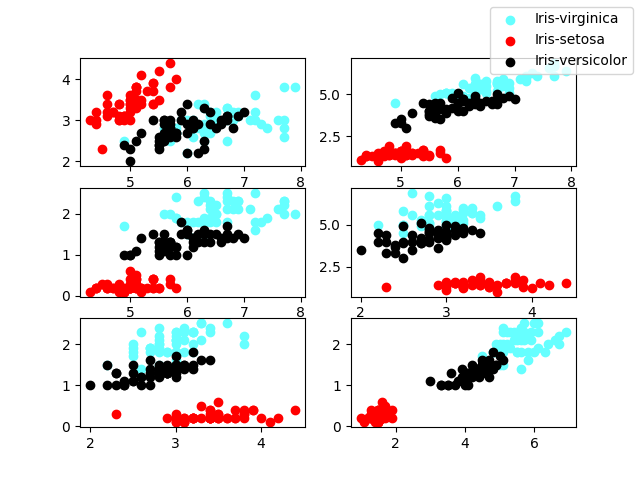
\includegraphics[width=10cm]{virginica_setosa_versicolor.png}
\end{figure}

From these images, we observe that the attributes of virginica
and versicolor are not linearly separable, as they both overlap 
any possible linear decision boundary. However, we can see that 
the other two species pairs have clear linear decision boundaries
between their attributes. Running the program multiple times
gave the following results for each species pair (max\_iter=1000):
\subsection*{versicolor vs setosa}
\begin{minted}{python}
Perceptron: 2.62*x_0 + 4.69*x_1 + -8.63*x_2 + -3.97*x_3 + 1.87 = 0
Accuracy: 1.0

Perceptron: 3.42*x_0 + 6.09*x_1 + -12.83*x_2 + -6.17*x_3 + 1.87 = 0
Accuracy: 1.0

Perceptron: 0.92*x_0 + 0.39*x_1 + -2.73*x_2 + -1.97*x_3 + 0.87 = 0
Accuracy: 1.0

Perceptron: 1.32*x_0 + 0.29*x_1 + -3.03*x_2 + -1.87*x_3 + 0.87 = 0
Accuracy: 1.0
\end{minted}
\subsection*{setosa vs virginica}
\begin{minted}{python}
Perceptron: -0.38*x_0 + -4.31*x_1 + 6.27*x_2 + 2.63*x_3 + -0.13 = 0
Accuracy: 1.0

Perceptron: -1.48*x_0 + -9.41*x_1 + 11.17*x_2 + 3.63*x_3 + -1.13 = 0
Accuracy: 1.0

Perceptron: 0.02*x_0 + -5.11*x_1 + 5.67*x_2 + 2.43*x_3 + -0.13 = 0
Accuracy: 1.0

Perceptron: -0.28*x_0 + -4.51*x_1 + 5.97*x_2 + 2.33*x_3 + -0.13 = 0
Accuracy: 1.0
\end{minted}
\subsection*{virginica vs versicolor}
\begin{minted}{python}
Perceptron: 54.42*x_0 + 54.89*x_1 + -52.53*x_2 + -167.87*x_3 + 61.87 = 0
Accuracy: 0.9

Perceptron: 11.92*x_0 + 4.89*x_1 + -14.93*x_2 + -12.67*x_3 + 4.87 = 0
Accuracy: 0.94

Perceptron: 34.82*x_0 + 152.69*x_1 + -107.43*x_2 + -161.27*x_3 + 150.87 = 0
Accuracy: 0.92

Perceptron: 61.22*x_0 + 80.29*x_1 + -109.73*x_2 + -145.57*x_3 + 231.87 = 0
Accuracy: 0.88
\end{minted}

The accuracy is maximum for all species pairs excluding 
virginica/versicolor. The coefficients for virginica/versicolor 
are exceptionally large compared to those of the other two 
pairs.

\end{solution}

\end{document}
